% Three-way concordance: Claude / GPT / Human on the FP subset.
% Schematic for the inter-judge concordance appendix.
\begin{figure}[t]
\centering
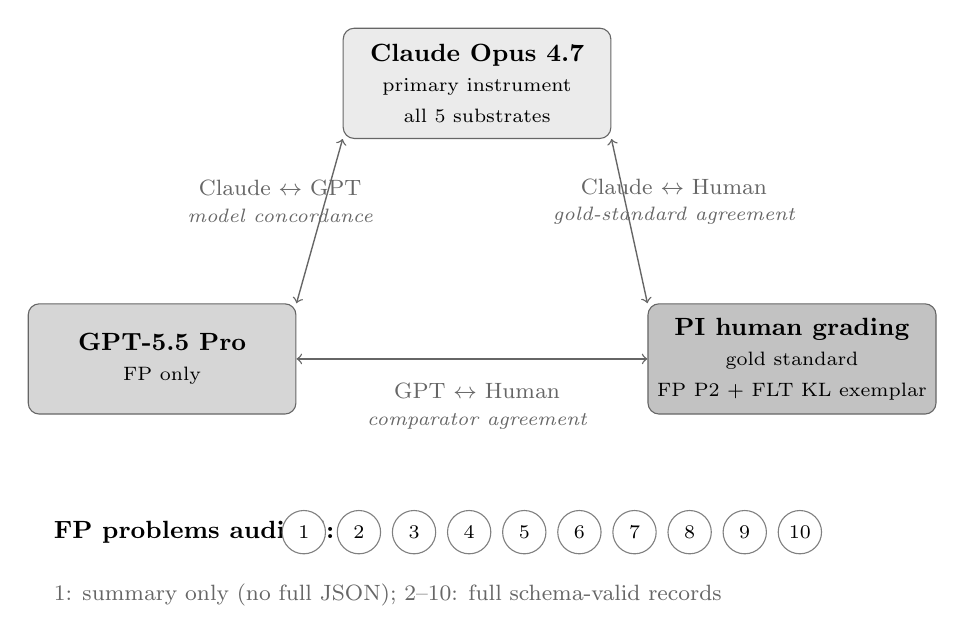
\begin{tikzpicture}[
  font=\small,
  judge/.style={
    rectangle, rounded corners=4pt, draw=black!60,
    minimum width=3.4cm, minimum height=1.4cm, align=center
  },
  jclaude/.style={judge, fill=black!8},
  jgpt/.style={judge, fill=black!16},
  jhuman/.style={judge, fill=black!24},
  arrow/.style={-{Latex[length=2mm]}, black!70, line width=0.5pt},
  pair/.style={<->, black!60, line width=0.5pt},
  prob/.style={
    circle, draw=black!50, fill=white,
    minimum size=0.55cm, font=\scriptsize, inner sep=0pt
  },
]

% Three judges arranged as a triangle
\node[jclaude] (claude) at (0, 3.5)
  {\textbf{Claude Opus 4.7}\\\scriptsize primary instrument\\\scriptsize all 5 substrates};
\node[jgpt] (gpt) at (-4, 0)
  {\textbf{GPT-5.5 Pro}\\\scriptsize FP only};
\node[jhuman] (human) at (4, 0)
  {\textbf{PI human grading}\\\scriptsize gold standard\\\scriptsize FP P2 + FLT KL exemplar};

% Pairwise comparisons
\draw[pair] (claude.south west) -- (gpt.north east);
\draw[pair] (claude.south east) -- (human.north west);
\draw[pair] (gpt.east) -- (human.west);

% Pair labels
\node[font=\footnotesize, black!60, align=center] at (-2.5, 2.0)
  {Claude $\leftrightarrow$ GPT \\ \scriptsize\itshape model concordance};
\node[font=\footnotesize, black!60, align=center] at (2.5, 2.0)
  {Claude $\leftrightarrow$ Human \\ \scriptsize\itshape gold-standard agreement};
\node[font=\footnotesize, black!60, align=center] at (0, -0.6)
  {GPT $\leftrightarrow$ Human \\ \scriptsize\itshape comparator agreement};

% Per-problem strip below
\node[font=\small\bfseries, anchor=west] at (-5.5, -2.2) {FP problems audited:};
\foreach \i/\x in {1/-2.2, 2/-1.5, 3/-0.8, 4/-0.1, 5/0.6, 6/1.3, 7/2.0, 8/2.7, 9/3.4, 10/4.1} {
  \node[prob] at (\x, -2.2) {\i};
}
\node[font=\footnotesize, anchor=west, black!60] at (-5.5, -3.0)
  {1: summary only (no full JSON); 2--10: full schema-valid records};

\end{tikzpicture}
\caption{Three-way inter-judge concordance design for the First-Proof subset.
The Discovery Tetrad audit's primary instrument is Claude Opus 4.7, applied
uniformly to all five substrates. To measure inter-judge reliability, the
First-Proof problems were also independently audited by GPT-5.5 Pro and
graded by hand by the authors using a structured exemplar protocol. The
three pairwise agreement statistics (Claude $\leftrightarrow$ GPT,
Claude $\leftrightarrow$ Human, GPT $\leftrightarrow$ Human) populate the
concordance appendix; the human grade is treated as the gold standard.
Problem~1 has only a Markdown summary (no full structured JSON) on the
GPT-judge side; Problems 2--10 carry full schema-valid records.}
\label{fig:concordance}
\end{figure}
